\documentclass[9pt,twocolumn,twoside]{pnas-report}

\templatetype{pnasresearcharticle}

\usepackage{lipsum}

\title{KeyNet: keyboard layout optimization using network analysis and genetic algorithms}

\author[a,1]{Arhar Anže}
\author[a]{Kostanjšek Kristjan}
\author[a]{Ločičnik Nejc}

\affil[a]{University of Ljubljana, Faculty of Computer and Information Science, Ve\v{c}na pot 113, SI-1000 Ljubljana, Slovenia}

\leadauthor{Arhar Anže}

\authordeclaration{All authors contributed equally to this work.}
\correspondingauthor{\textsuperscript{1}To whom correspondence should be addressed. E-mail: aa3178@student.uni-lj.si.}

\begin{abstract}
In our report we introduce a novel approach to keyboard layout optimization using network analysis and genetic algorithms.
We constructed a weighted directed graph based on text samples and used centrality measures to create a baseline layout.
This initial layout was then optimized with genetic algorithms.
Evaluations, visualized through heatmaps, highlight the efficiency of our layouts compared to traditional ones like QWERTY and Dvorak.
While limited to the text of "War and Peace," our framework is adaptable to various text types, offering potential for task-specific optimization.
Future work would focus on unbiased evaluation methods and user testing to validate real-world effectiveness.
\end{abstract}

\dates{The manuscript was compiled on \today}
\doi{\href{https://ucilnica.fri.uni-lj.si/course/view.php?id=183}{Introduction to Network Analysis} 2023/24}

\begin{document}

\maketitle
\thispagestyle{firststyle}
\ifthenelse{\boolean{shortarticle}}{\ifthenelse{\boolean{singlecolumn}}{\abscontentformatted}{\abscontent}}{}

\dropcap{A}s we know, typing speed is one of the most important quality measures for every dedicated computer science engineer.
A significant factor influencing typing speed is the keyboard layout used.
The most popular keyboard layouts today include QWERTY, AZERTY, Dvorak, and Colemak.
Of these, QWERTY remains the dominant layout, despite its origins dating back to the 1870s.
While QWERTY has been incrementally improved over time, resulting in a relatively optimal layout given its historical constraints, there is potential for entirely different layouts that could significantly enhance typing speed and comfort.
Moreover, the optimal keyboard layout can vary depending on the specific typing task, such as coding versus writing a novel.
The layout can also vary significantly depending on the language being typed.

This paper aims to optimize keyboard layouts tailored to specific types of text, including programming code, English language text, Slovenian language text, and more.
Additionally, we seek to evaluate the efficiency of the layouts we developed and compare them to current popular keyboard layouts, such as QWERTY and Dvorak.
By doing so, we hope to identify layouts that offer superior performance for specific tasks, ultimately enhancing typing speed and comfort for users.
Our main contribution is visualized using a key frequency heatmap in Figure \ref{fig:main_contributions}.

\begin{figure}[t]\centering%
    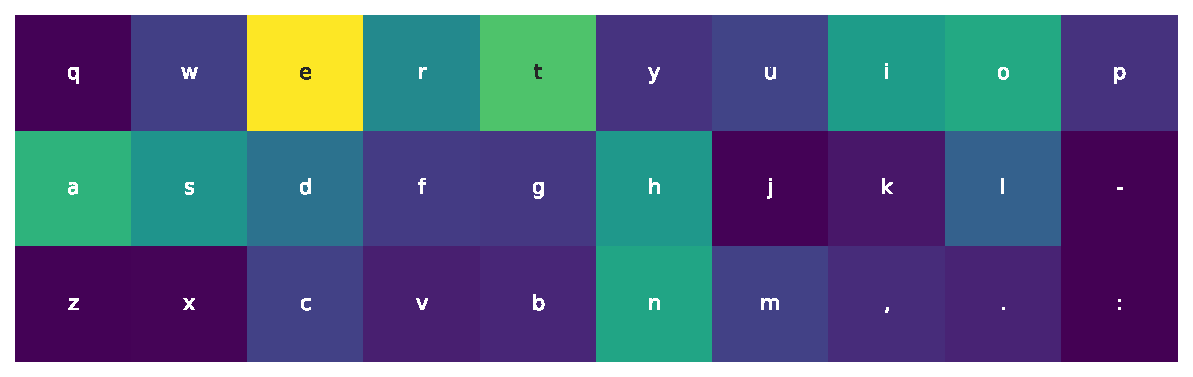
\includegraphics[width=0.9\linewidth]{fig/qwerty}
    \small{QWERTY}
    \vskip8pt
    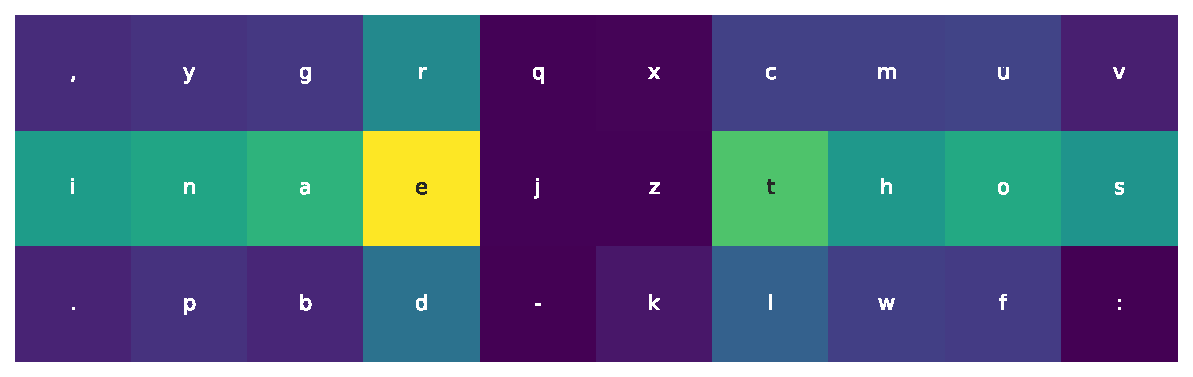
\includegraphics[width=0.9\linewidth]{fig/genetic}\\
    \small{Ours}
    \caption{Our finalized keyboard layout compared to the standard QWERTY layout.}
    \label{fig:main_contributions}
\end{figure}

\section*{Related work}

Keyboard layout optimization is a popular problem with no unique solution.
Most approaches utilize genetic algorithms or a combination of genetic algorithms and deep learning to tackle this issue.
Notable examples include works by Švigelj \cite{svigelj2019}, Nivasch \& Azaria \cite{NiAz2021, NiAz2023}, Onsorodi \& Korhan \cite{onsorodi2020}, and Khan \& Deb \cite{KhDe2023}.
Additionally, two articles specifically focus on optimizing keyboard layouts based on the language being typed: Pacheco et al. \cite{eniac} and Liao \& Choe \cite{ChCh2013}.

Genetic algorithms are particularly well-suited for this problem, which is why we partially incorporated them in our approach.
However, we found few articles leveraging network analysis for keyboard layout optimization.
Despite this, we believe network analysis can effectively establish a solid foundation for layout design.

\section*{Results}

Figure \ref{fig:layouts} visualizes the key frequency heatmaps for each keyboard layout.
As QWERTY was not designed for modern typing needs, the layout is not ergonomic and most used keys are spread across the whole keyboard.
Dvorak tries to mitigate this by placing most frequent keys on the home row, but ignores the finger strength which is highly tied with typing ergonomics.

Comparing our generated layouts to QWERTY and Dvorak, we can distinctly see the optimization profile employed in the generation process.
Degree centrality and genetically optimized layouts feature prominent home row usage with the most used keys laying under the stronger fingers.
The genetically optimized layout also features better bigram allocation.
Keys that are most frequently used are positioned together, forming bigram clusters that enable fast typing speeds.
The least used symbols lie at the edges of the keyboard and at the center two rows, as expected.

\begin{table}[h]\centering%
	\caption{Table describing data or methods.}
	\begin{tabular}{lccccc}\toprule
	    & $n$ & $m$ & $\langle k\rangle$ & $\langle C\rangle$ & $\langle d\rangle$ \\\midrule
	    Fine network & $438\,920$ & $9\,742\,733$ & $44.4$ & $0.37$ & $6.19$ \\
	    Random graph & $438\,920$ & $9\,781\,609$ & $44.6$ & $0.00$ & $4.92$ \\\bottomrule
	\end{tabular}
	\label{tbl:example}
\end{table}

\lipsum[2-3]

\begin{figure}[t]\centering%
    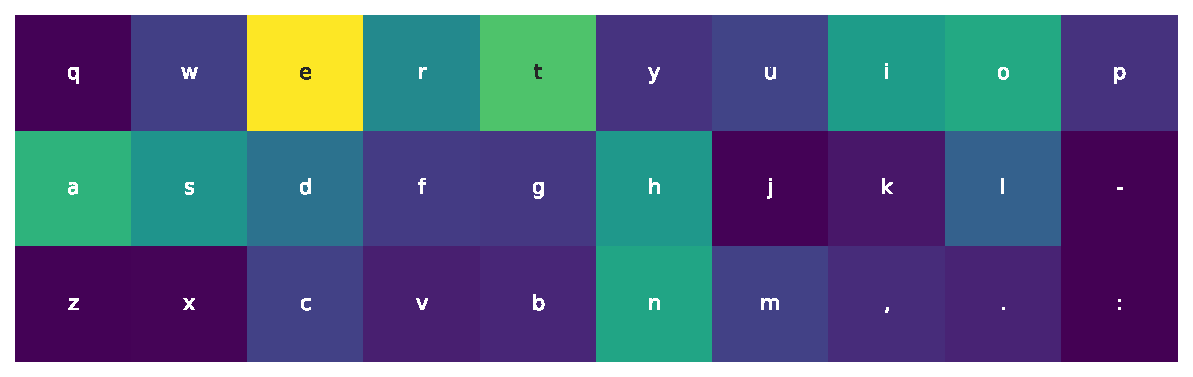
\includegraphics[width=0.9\linewidth]{fig/qwerty}
    \small{QWERTY}
    \vskip8pt
    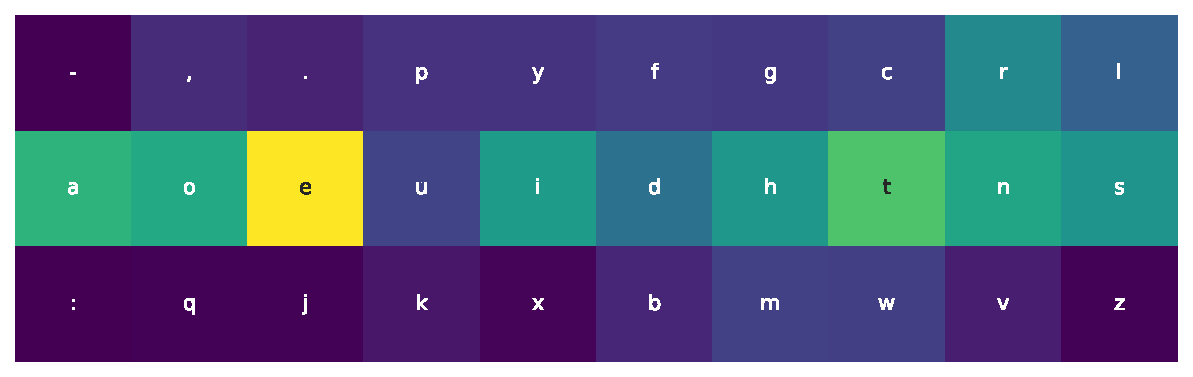
\includegraphics[width=0.9\linewidth]{fig/dvorak}
    \small{Dvorak}
    \vskip8pt
    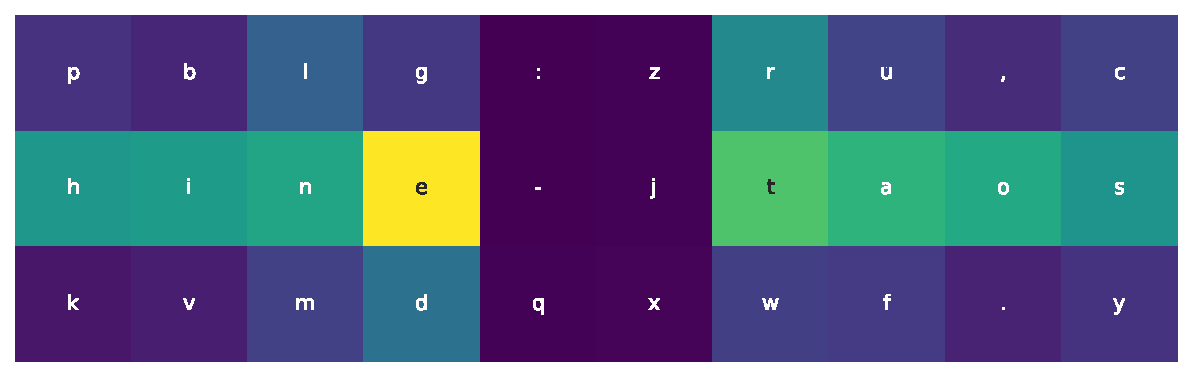
\includegraphics[width=0.9\linewidth]{fig/centrality}
    \small{Ours\,(degree centrality)}
    \vskip8pt
    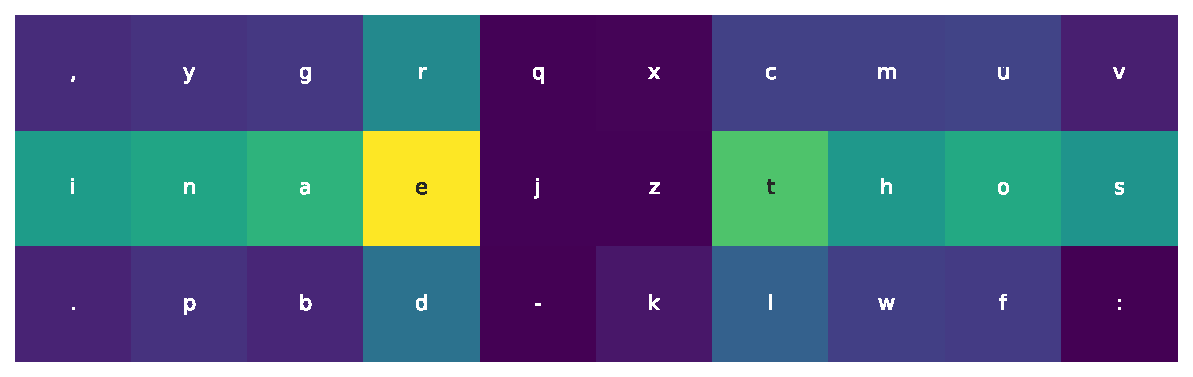
\includegraphics[width=0.9\linewidth]{fig/genetic}
    \small{Ours\,(genetic algorithm)}
    \caption{Keyboard layouts visualized using key frequency heatmaps.}
    \label{fig:layouts}
\end{figure}

\lipsum[4-6]

\section*{Discussion}

Due to time limitations, we were able to test our keyboard layout optimizer only on the War and Peace novel.
However, we have developed a flexible framework that allows for easy testing on various types of text (so the optimization of e.g. keyboard used for writing programming code would be effortless).
This capability opens up the possibility for text-specific keyboard optimization, catering to different user needs.

One limitation of our current evaluation method is that we only visualizes the heatmap based on key frequency.
We do not visualize the relationships between different keys, as such a visualization would be overly complex and unclear.
A potential future improvement would be to develop an unbiased method for evaluating different keyboards that takes key relationships into account without compromising clarity.

Additionally, we did not have sufficient time to test the keyboards ourselves.
Future work should include thorough user testing to validate the effectiveness and comfort of the optimized layouts in real-world scenarios.
This will provide practical insights and further refine our optimization framework.

{\small

\section*{Methods}

To address the challenge of optimizing keyboard layouts, we employed an ortholinear keyboard.
We began by utilizing network analysis to construct a weighted directed graph, where the nodes represented keys and the links represented the frequency of successive key presses.
With the analysis of this graph we built the foundation for our initial layout.
Subsequently, we applied genetic algorithms to refine and optimize this layout to the greatest extent possible.
Although we did not have sufficient time to personally become fully proficient with the new layouts, we evaluated them using other metrics, such as the distance our fingers traveled while typing various texts.

In this section, we will detail the process of designing the keyboard layout.
First, we gather text samples (e.g. books or programming code) and preprocess them by removing unnecessary symbols, spaces, line breaks, and tabs.
This preprocessing results in a string composed solely of the 26 English alphabet letters and 4 additional symbols: period, comma, hyphen, and a colon.
This gives us a total of 30 characters, suitable for our 3 x 10 ortholinear keyboard.
Next, we use this preprocessed text to construct a graph, employing network analysis methods to establish the foundation of our keyboard layout.
Finally, this foundational layout is subjected to a genetic algorithm to achieve full optimization.

\subsection*{Network analysis}

To build a naive baseline layout we need to evaluate node importance with the help of techniques from network analysis.
Since what we are working with is a directed weighted (almost) fully connected graph with 30 nodes, we are very limited with the types of methods we can make use of.
What we can use are centrality measures, which generally make use of the pathways in the graph, that are in our case weighted based on bigram occurrence.

\subsubsection*{Node importance}

The metrics used were: degree centrality, eigenvector centrality, betweenness centrality, closeness centrality and page rank.
Of these, closeness had to be manually implemented to account for weights since the NetworkX python library implementation didn't.
Betweenness, closeness and page rank also needed an additional weight change, since what they look for is the shortest path, in our case least weighted pathways.
In these cases the weights were recalculated using the following equation: $1 - \text{edge}_\text{weight}$.

What we are looking for is a ranking of importance, so we added an additional metric, which combines all of these.
We simply averaged the rank each symbol gets with these metrics.

\subsubsection*{Splitting the graph}

We obviously type with two hands so we need to split the graph into two subgraphs, one for each hand.
We can't simply randomly split the nodes.
We want to optimize the layout to reduce the amount of time we spend typing.
Ideally, we want bigrams to be typed interchangeably with both hands, meaning we want the sum of edge weights between the two subgraphs to be as high as possible.

We can achieve this by trying to balance the sum of inner weights of the two subgraphs.
We got an approximation of this by splitting the nodes based on the weighted degree centrality.
The split was made interchangeably between the two subgraphs, e.g. node with the highest degree centrality in subgraph 1, node with second highest degree centrality in subgraph 2, 3rd node in subgraph 1 again, etc.

This approximation is then optimized by randomly swapping the nodes between the two subgraphs.
If the node swap leads to an improvement in the balance, we keep it, otherwise we swap the nodes back.

This optimization always converges, so that we have approximately a quarter of the weights within the internal connections of each subgraphs and approximately half of the weights within the edges connecting the two subgraphs.

\subsubsection*{Base layout}

Once we split the nodes on two subgraphs, we can start building the keyboard layout.
Since we want each hand to be in charge of one half of the keyboard, we can consider each half of the keyboard completely independent from the other.

We start building the layout from the home row.
We first place the 4 most important nodes by the chosen metric (one of the centrality measures or their combined ranking) on the keys where we rest each of the fingers.
The placing is done in order of finger dexterity and reach: index, middle, ring and little finger.

Once we fill the most important key positions, we need to fill the keys directly above and below them.
Here, we take into consideration that we want to punish using a single finger two times in a row (excluding pressing the same key twice).
We can score each of the remaining nodes by the following score: sum of weights to the other keys on the home row minus the weight to the key directly above or below.
We place the first position of this scoring metric on the top row and the second place on the bottom row.
We do this in the same order as placing keys on the home row, index finger first, little finger last.

Finally, we are left with row next to the index finger row, which requires lateral movement from the index finger.
Here, we again score the remaining keys based on the sum of weights from the rest of the placed keys minus the sum of weights to the keys placed in the index finger row.
The first position is placed on the home row, the second above it and the last, least important key below it.

We do this procedure for the nodes of both subgraphs, flip one of the produced layouts and concatenate them to get the full baseline keyboard layout.

\subsection*{Genetic algorithms}

As key layout optimization is a permutation problem, we decided to optimize our layout using a genetic algorithm.
By defining the problem in this way, we can easily design a cost function that is defined only using matrix operations.
This allows us to speed up the computations significantly, resulting in better layout designs.

Each gene in the population is represented as a permutation.
Our goal is to find the optimal permutation of keys that minimizes the cost function $c$.
In this section, the function $\text{diag}$ refers to creating a diagonal matrix from a vector $v \in \mathbb{R}^n$:

\begin{equation}
    \text{diag}(v) = D \in \mathbb{R}^{n \times n}, \text{ where } D_{i,j} = \begin{cases}
        v_i, & i = j\\
        0, & \text{otherwise}
    \end{cases}
\end{equation}
We define the cost function $c$ using the following matrices:
\begin{itemize}
    \item Probability matrix $P$ contains the bigram probabilities $p$
    \begin{equation}
        P_{i,j} = p_{i,j}
    \end{equation}
    \item Markov chain transposition matrix $A$ of the network is used to calculate the stationary probability vector $pi$
    \begin{equation}
        \pi A = \pi
    \end{equation}
    \item Preferred position matrix $R$ is a diagonal matrix of key importances
    \begin{equation}
        R = \text{diag}\left(\text{vec}\left(
        \begin{bmatrix}
            2 & 3 & 4 & 5 & 1 & 1 & 5 & 4 & 3 & 2\\
            6 & 7 & 8 & 9 & 2 & 2 & 9 & 8 & 7 & 6\\
            2 & 3 & 4 & 5 & 1 & 1 & 5 & 4 & 3 & 2
        \end{bmatrix}^T\right)\right)
    \end{equation}
    \item Distance matrix $D$ contains the physical distances between the keys
    \begin{equation}
        D_{i,j} = \sqrt{(x_i - x_j)^2 + (y_i - y_j)^2}
    \end{equation}
    \item Same finger bigram matrix $F$ groups keys assigned to the same finger
    \begin{equation}
        g = \text{vec}\left(
        \begin{bmatrix}
            1 & 2 & 3 & 4 & 4 & 5 & 5 & 6 & 7 & 8\\
            1 & 2 & 3 & 4 & 4 & 5 & 5 & 6 & 7 & 8\\
            1 & 2 & 3 & 4 & 4 & 5 & 5 & 6 & 7 & 8
        \end{bmatrix}^T\right)
    \end{equation}
    \begin{equation}
        F_{i,j} =
        \begin{cases}
            1, & g_i = g_j\\
            0, & \text{otherwise}
        \end{cases}
    \end{equation}
\end{itemize}
Cost $c$ is defined using a weighted sum of the permuted matrices which is finally element-wise summed into a single number
\begin{equation}
    C(E) = E P \cdot (w_1 F + w_2 D) - w_3\text{diag}(E \pi)R
\end{equation}
\begin{equation}
    c = \sum_i \sum_j C_{i,j}
\end{equation}
Using a weighted sum allows us to assign more weight to some scores and less to other.
All of the aforementioned matrices are displayed in Figure \ref{fig:matrices}.

\begin{figure}[t]\centering%
	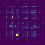
\includegraphics[width=0.3\linewidth]{fig/p}
	
\includegraphics[width=0.3\linewidth]{fig/pi}
        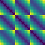
\includegraphics[width=0.3\linewidth]{fig/d}\\
        \vspace{0.2em}
        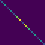
\includegraphics[width=0.3\linewidth]{fig/r}
        
\includegraphics[width=0.3\linewidth]{fig/f}
        
\includegraphics[width=0.3\linewidth]{fig/e}
	\caption{Matrices visualized in the following order from left to right and top to bottom: $P$, $\text{diag}(\pi)$, $D$, $R$, $F$, and $E$.}
        \label{fig:matrices}
\end{figure}

In each generation we keep the 10 \% of the previous population with the lowest cost.
Next 50 \% of the genes according to their cost are only mutated.
Mutations are represented using a random swap of two elements.
Other 40 \% of genes are a recombination of all genes from the previous population.
This is achieved using the partially mapped crossover (PMX) algorithm \cite{goldberg2014alleles}, which swaps parts of two permutations in a way that keeps a part of the original permutation.
Candidates for recombination are selected according to their cost - lower cost has a higher probability of being selected and higher cost has a lower probability of being selected.
The mutation and crossover procedure operate only inclusively on homerow keys or other keys.
This limitation is added to keep similar structure to the layout designed using network analysis.

\subsection*{Evaluation}

We constructed our keyboard layouts using text from War and Peace by Leo Tolstoy.
Evaluating the effectiveness of these keyboards presents a unique challenge.
One potential method of evaluation involves using the cost function described in the previous subsection.
However, this approach could introduce bias, as the keyboards were optimized based on this very cost function.

To avoid this bias, we decided to take a different approach.
We visualized each keyboard layout with a heatmap representing the frequency of key presses.
By analyzing these heatmaps, we can gain insights into the distribution of key usage and provide qualitative commentary on the efficiency and comfort of the layouts.

}

% \acknow{The authors would like to\dots}

% \showacknow{}

\bibliography{bibliography}

\end{document}
